%% isiMonitor3d — Master's-thesis article (CONFIDENTIAL, ISITEC)
%% Typeset with the Rho class v3.0.1. Build:
%%   ~/miniforge3/envs/tex/bin/tectonic isimonitor3d.tex
\documentclass[9pt,a4paper,twocolumn]{rho-class/rho}
\usepackage[english]{babel}

% Math-font repair for the tectonic bundle: the class's stix2 (Type-1) math
% setup is incomplete in this bundle (fallbacks drop \times, minus, primes,
% \mid). unicode-math + the bundled STIX Two Math OTF restores the SAME
% intended typeface with a complete glyph set. Reported as a deviation.
\usepackage{amsmath}
\usepackage{unicode-math}
\setmathfont{STIXTwoMath-Regular.otf}

\addbibresource{isimonitor3d.bib}

%----------------------------------------------------------
% Title
%----------------------------------------------------------

\doctype{Research Article}
\title{A Modular Real-Time Multi-Camera Vision System for Metric 3D Monitoring of Warehouse Logistics}
\subtitle{Synthetic-Data-Assisted Detection, Dual-Method Geometric Localization, and Edge Deployment}
\runningtitle{Modular Metric 3D Vision System for Warehouse Logistics}

%----------------------------------------------------------
% Authors, Affiliations and dates
%----------------------------------------------------------

\author[a,1]{Abdullahi Adewale ATANDA}
\author[b,2]{Yang NIU}

\affil[a]{Universit\'e Grenoble Alpes, Grenoble, France}
\affil[b]{ISITEC International, France}

\dates{Compiled on \today}

%----------------------------------------------------------
% Corresponding author-, Document- information
%----------------------------------------------------------

\corres{\textcolor{red}{\textbf{CONFIDENTIAL --- This work describes a private industrial project of ISITEC International, France.}}}
\corres{\textsuperscript{1}Corresponding author. Email: \href{mailto:abdullahi.atanda@univ-grenoble-alpes.fr}{abdullahi.atanda@univ-grenoble-alpes.fr}}
\corres{\textsuperscript{2}Industrial mentor. Email: \href{mailto:y.niu@isitec-international.com}{y.niu@isitec-international.com}}

\docinfo{Master's-thesis article, Universit\'e Grenoble Alpes. Submitted to the examination committee; journal target: Computers in Industry (Elsevier).}

\journalname{Submitted to: Computers in Industry}
\journal{Computers in Industry (Elsevier)}
\theday{\today}

%----------------------------------------------------------
% Abstract and Keywords
%----------------------------------------------------------

\begin{abstract}
Infrastructure-side warehouse monitoring requires real-time object positions in metric coordinates with persistent identities for vehicle fleets and warehouse management systems. Existing vision systems operate mainly in image space and require site-specific calibration and detector retraining, increasing deployment cost. This paper presents isiMonitor3d, a modular industrial vision system comprising five modules from operator-guided calibration to machine-consumable data delivery. A single calibration supports two complementary localization methods: always-on ground-plane homography and on-demand stereo triangulation, both sharing a common identity space.

Validated on a deployed dual-camera system under full production load, isiMonitor3d achieved a 40.3\,ms median and 78.1\,ms 95th-percentile capture-to-publish latency, well below the 200\,ms target. Calibration reached a 1.621\,px bundle-adjustment residual (target $\leq 2$\,px), while the best detector achieved 0.977 box mAP@0.5 on the validation set. A controlled ablation showed that synthetic images generated from 53 real photographs cannot replace real training data (0.223 vs.\ 0.941 box mAP@0.5 on real frames), although they provided a modest recall improvement ($+0.050$) when used for augmentation. These results demonstrate that an integrated calibration-to-delivery pipeline can deliver reliable real-time metric monitoring on a single edge GPU.
\end{abstract}

\keywords{industrial vision system, multi-camera tracking, camera calibration, synthetic training data, edge inference, warehouse logistics}

%----------------------------------------------------------

\begin{document}

    \maketitle
    \thispagestyle{firststyle}

%----------------------------------------------------------

\section{Introduction}

\rhostart{W}arehouse operations are automating rapidly, and with automation comes a new monitoring problem: automated guided vehicles (AGVs) and autonomous mobile robots increasingly share floor space with people, forklifts, and moving goods, under safety requirements codified for driverless industrial trucks in ISO 3691-4 \cite{iso36914}. Vehicle-mounted safety sensors protect the immediate surroundings of each vehicle, but site-level questions --- who is inside a danger zone, which storage zone holds which pallets, whether a pallet left a zone loaded or empty --- require infrastructure-side perception: fixed cameras observing the shared floor and reporting its state to the fleet controllers and warehouse management systems that act on it. Deep-learning computer vision has been identified as a key enabler for exactly these warehousing tasks, including entity re-identification, multi-view localization on the shop floor, and category-agnostic segmentation of bin items for robotic grasping \cite{rutinowski2022potential}.

For such a system's output to be actionable, pixel-space perception is insufficient. A fleet controller cannot consume bounding boxes in one camera's image plane; it needs object positions in metric world coordinates, identities that persist over time so that zone entries, exits, and dwell times are attributable to individual objects, and the zone-level events derived from both. Conventional CCTV analytics --- detections, counts, heatmaps --- live in image space, cannot express an inter-object distance in meters, and therefore cannot directly support safety monitoring or vehicle coordination.

Deploying such a system in an industrial warehouse introduces several practical challenges beyond the perception task itself. The system must operate in real time on a single edge GPU without cloud connectivity, support operator-friendly installation and maintenance, tolerate camera failures mid-shift, and adapt to site-specific layouts and object appearances for which no public datasets exist.

The research literature addresses these needs in four largely separate bodies of work. \textbf{Multi-camera localization.} Multi-camera people tracking is a mature field with dedicated surveys \cite{iguernaissi2019people}; the probabilistic occupancy map of Fleuret et al.\ demonstrated metrically accurate ground-plane tracking from few synchronized cameras \cite{fleuret2008multicamera}, more recent bird's-eye-view methods such as MVDet project learned features onto the ground plane before detection \cite{hou2020mvdet}, and tracking-by-detection has converged on Kalman-filter motion models with Hungarian association \cite{bewley2016sort}, refined by ByteTrack's two-pass association over high- and low-confidence detections \cite{zhang2022bytetrack}. However, these works focus on benchmark datasets and do not address industrial deployment, calibration workflows, or fault tolerance.

\textbf{Calibration and geometry.} The geometric machinery itself is textbook material \cite{hartley2004multiple}: planar-target camera calibration \cite{zhang2000flexible}, its fiducial infrastructure (AprilTag \cite{olson2011apriltag}, ArUco/ChArUco \cite{garridojurado2014aruco}), plane-induced homographies, and direct linear transformation (DLT) triangulation. Existing work, however, typically treats ground-plane homography and multi-view triangulation as alternative localization methods --- the former cheap but confined to floor contact, the latter fully 3D but requiring synchronized calibrated views. To our knowledge, no deployed system described in the literature we reviewed integrates both from a single calibration while maintaining a shared identity space.

\textbf{Detection.} Real-time detection evolves along two lines --- the single-stage YOLO family from its origin \cite{redmon2016yolo} through its surveyed evolution \cite{terven2023comprehensive} to the NMS-free, edge-oriented YOLO26 generation \cite{jocher2026yolo26}, and the detection-transformer line from DETR \cite{carion2020detr} through real-time variants \cite{zhao2024rtdetr} to the fine-tuning-oriented RF-DETR \cite{robinson2025rfdetr} --- while portable inference runtimes (ONNX Runtime \cite{onnxruntime}, TensorRT \cite{tensorrt}) make these models deployable on heterogeneous edge hardware through a single exchanged model artifact. Existing detector research, however, emphasizes benchmark accuracy and throughput rather than deployment-aware inference that exploits static scene priors --- in a fixed-camera installation, most of every frame never changes and activity concentrates in known zones.

\textbf{Synthetic training data.} On the data side, synthetic imagery has progressed from domain randomization in rendered scenes \cite{tobin2017domain} to diffusion-based generation: SDXL provides photorealistic synthesis \cite{podell2023sdxl}, ControlNet constrains it with geometric control maps so that labels can be derived by construction \cite{zhang2023controlnet}, and low-rank adaptation (LoRA), introduced for language models \cite{hu2022lora} and since applied to diffusion backbones, adapts the generator to a specific object class from a few dozen examples. Although these techniques have shown promise on public datasets, their effectiveness within a complete industrial monitoring pipeline remains largely unvalidated.

Across the reviewed literature, we did not find a complete industrial vision system integrating operator-guided calibration, synthetic-data-assisted detector training, metric multi-camera localization, and machine-consumable delivery into a single measured pipeline. Bridging this integration gap is the objective of this work.

Closing the gap matters for three practical reasons. \textbf{Safety:} the safety functions ISO 3691-4 requires of driverless trucks are vehicle-centric \cite{iso36914}; infrastructure-side metric tracking complements them with continuous site-level supervision --- person positions in meters, evaluated against danger-zone polygons and delivered to the fleet controller before any vehicle's own sensors are in range. \textbf{Inventory and flow:} the same tracks give warehouse management systems a live, per-zone view of goods, zone entry and exit events, and pallet empty/full state --- signals otherwise obtained by manual scanning. \textbf{Deployment economics:} lightweight calibration from printed boards and one mid-range GPU keep the hardware side modest, while synthetic imagery generated from on the order of fifty real photographs of a class can augment --- though, on our own ablation evidence, not replace --- the per-site collection and annotation campaign (Section 3.4).

This article describes isiMonitor3d, a complete industrial vision pipeline built to a warehouse-logistics customer specification (cahier des charges) whose acceptance targets are sub-200\,ms capture-to-publish latency (95th percentile), homography reprojection error at most 2\,px, per-view triangulation reprojection error gated at 5--8\,px, detection mAP@0.5 of at least 0.90, and pallet empty/full classification precision/recall of at least 0.95/0.93. The system spans five modules --- operator-guided calibration, a perception producer, a metric-geometry engine, a synthetic-data/training pair, and a communication gateway --- and offers two localization modes: continuous 2D floor tracking by ground-plane homography and on-demand 3D tracking by stereo triangulation, delivered as versioned JSON over UDP and MQTT with a polling REST gateway for AGV fleet controllers.

The main contributions of this work are:

\begin{enumerate}
    \item A \textbf{modular five-module architecture} with frozen communication contracts, enabling single-decode multi-consumer processing and measured real-time performance (capture-to-publish latency of 40\,ms p50 / 78\,ms p95 under full production load on one 12\,GB edge GPU).
    \item A \textbf{dual-method localization framework} combining always-on ground-plane homography and on-demand stereo triangulation from a shared calibration and identity space.
    \item An \textbf{operator-guided calibration workflow} (isical) achieving a 1.62\,px reprojection consensus on the deployed rig using printed calibration boards only.
    \item A \textbf{synthetic-data generation pipeline} (isiGen: SDXL + ControlNet + LoRA), together with a quantitative evaluation of synthetic versus real training data for industrial object detection (Section 3.4).
\end{enumerate}

The remainder of the article is organized as follows. Section 2 presents the materials and methods: background on the underlying architectures and tools (2.1), system architecture and wire contracts (2.2), calibration (2.3), perception and detection models (2.4), the geometric core (2.5), synthetic data generation (2.6), and communication and deployment (2.7). Section 3 reports experimental results against the acceptance targets --- calibration accuracy, detector accuracy, runtime performance, and synthetic geometric-accuracy bounds. Section 4 discusses these results, including the design decisions the measurements justify, and states the limitations of the current validation. Section 5 concludes and outlines future work.

\section{Materials and Methods}

\subsection{Background: underlying architectures and tools}

isiMonitor3d integrates components from six complementary research areas: vision inference, multi-object tracking, projective geometry, synthetic-data generation, machine-consumable data delivery, and edge deployment. This subsection summarizes the specific architectures the system builds on --- the two detector families (2.1.1--2.1.2), the generative stack of the synthetic-data pipeline (2.1.3--2.1.6), and the messaging protocol of the delivery layer (2.1.7) --- and closes with the tracking, geometric, and runtime foundations (2.1.8). Each summary is limited to the architectural properties the system directly exploits, followed by the concrete form the component takes in isiMonitor3d.

\subsubsection{YOLO26 --- single-pass instance segmentation}

The YOLO family frames detection as a single forward pass of a fully convolutional network that predicts classes and boxes densely over the image, trading the region-proposal stage of two-stage detectors for throughput \cite{redmon2016yolo}. Across its generations the family converged on a three-part structure \cite{terven2023comprehensive}: a convolutional backbone extracts features at several scales; a neck aggregates these features across pyramid levels, so that small and large objects are each predicted from feature maps of appropriate resolution; and a decoupled head regresses boxes and classifies objects in separate branches. The dense predictions of such one-stage detectors are redundant by construction and have historically required non-maximum suppression (NMS) --- a data-dependent, sequential post-processing step --- to select final detections.

YOLO26, the generation adopted here, removes this dependency: it is trained for end-to-end prediction, so the network emits a final detection set directly without NMS, and it drops the distribution-focal-loss regression module of earlier generations, simplifying the prediction head \cite{jocher2026yolo26}. Because this project exports the raw prediction head --- no decoding baked into the artifact --- the exported graph never contained NMS in any YOLO generation; the benefit the end-to-end head delivers here lies on the application side: detection decoding reduces to confidence filtering, coordinate un-letterboxing, and mask assembly, with no data-dependent suppression stage whose cost varies with scene density (the postprocessing cost breakdown of Section 3.3 reflects this). The release documentation additionally reports up to 43\,\% faster CPU ONNX inference for the nano variant relative to its YOLO11 predecessor \cite{jocher2026yolo26}. The instance-segmentation (\texttt{-seg}) variants extend the head with the prototype-based mask design introduced by YOLACT \cite{bolya2019yolact}: the network predicts one shared bank of prototype masks per image plus a small coefficient vector per detection, and each instance mask is the thresholded sigmoid of a linear combination of the prototypes --- adding segmentation at near-constant cost over detection.

In isiMonitor3d, the production detectors are YOLO26-seg models fine-tuned in the isidet trainer on the three-class warehouse corpus (Section 2.6): the headline \texttt{yolo26l-seg} (640\,px input; 0.977 box mAP@0.5 and 0.948 box mAP@0.5:0.95 on the validation split --- Section 3.1, \tabref{tab:t1}) and the deployed \texttt{yolo26n-seg}, which meets the accuracy target at a 320\,px input (0.962 / 0.895). Models are exported to ONNX (opset 17) with the raw prediction head, so box decoding and prototype-mask combination remain under application control (Section 2.4).

\subsubsection{RF-DETR --- detection transformer}

DETR recasts detection as direct set prediction \cite{carion2020detr}. A transformer encoder \cite{vaswani2017attention} processes the flattened feature map of a convolutional backbone; in the decoder, a fixed set of learned object queries cross-attends to the encoded image features, each query producing one (class, box) prediction. Training assigns predictions to ground-truth objects one-to-one by bipartite Hungarian matching, and the resulting loss teaches the network itself to suppress duplicates --- no anchors, no NMS. The original formulation, however, converged slowly and paid quadratic attention cost over dense feature maps. Deformable DETR addressed both by replacing full attention with multi-scale deformable attention, which samples a small learned set of points around each reference location \cite{zhu2021deformable}, and subsequent real-time DETRs such as RT-DETR added efficient hybrid encoders and improved query selection, reaching YOLO-class speed \cite{zhao2024rtdetr}.

RF-DETR continues this real-time line with a different emphasis: rather than proposing a single fixed architecture, it fine-tunes a pretrained base network and applies weight-sharing neural architecture search over the model's tunable dimensions, discovering accuracy--latency trade-offs per target dataset and explicitly aiming at transferability of DETRs to domains far from the pretraining distribution \cite{robinson2025rfdetr}. This orientation toward fine-tuning on small, domain-specific datasets matches the per-site training regime of Section 1.

In isiMonitor3d, RF-DETR-seg is the alternative detector family behind the same \texttt{Detector} interface. The evaluated model is \texttt{rfdetr-medium-seg}, fine-tuned on the same corpus; it reads a fixed 432\,px square input, and its exported ONNX graph exposes three named outputs --- \texttt{dets} (normalized boxes), \texttt{labels} (per-query class logits), and \texttt{masks} (per-query mask logits) --- decoded without NMS. At its selected checkpoint it reaches 0.973 box mAP@0.5 and 0.938 box mAP@0.5:0.95 on the validation split (Section 3.1, \tabref{tab:t1}). Because both families serve the same detector interface, each deployment adopts whichever fine-tunes better on its data.

\subsubsection{SDXL --- latent diffusion}

In the denoising-diffusion formulation \cite{ho2020ddpm}, image generation inverts a gradual noising process: a fixed forward process corrupts a training image with Gaussian noise over many steps, and a network --- typically a UNet --- is trained to reverse the corruption step by step, so that sampling reconstructs an image from noise. Latent diffusion made this affordable at high resolution by moving denoising out of pixel space \cite{rombach2022ldm}: a variational autoencoder compresses images into a lower-dimensional latent space, the denoising UNet operates entirely on latents --- conditioned on text through cross-attention over the prompt's encoder embeddings \cite{vaswani2017attention} --- and the autoencoder's decoder maps the final latent back to pixels.

SDXL scales this recipe \cite{podell2023sdxl}: a UNet roughly three times larger than in earlier Stable Diffusion versions, text conditioning from two encoders whose embeddings are concatenated (OpenCLIP ViT-bigG and CLIP ViT-L), and additional conditioning on the original image size and crop coordinates of each training example, which allows training on the full dataset without discarding small images and suppresses cropping artifacts at sampling time.

In isiMonitor3d, SDXL is the generator of the isiGen synthetic-data pipeline (Section 2.6): the publicly released \texttt{stabilityai/stable-diffusion-xl-base-1.0} checkpoint, used with frozen weights and extended only through the two mechanisms described next --- spatial conditioning by ControlNet (2.1.4) and class specialization by LoRA (2.1.5).

\subsubsection{ControlNet --- spatial conditioning}

ControlNet adds spatial control to a pretrained text-to-image diffusion model without retraining it \cite{zhang2023controlnet}. The architecture duplicates the encoder and middle blocks of the base UNet into a trainable copy that receives, in addition to the latent, a spatial control map --- a depth map, edge map, or pose skeleton aligned with the target image. The copy's outputs are injected into the frozen base network through zero-initialized $1 \times 1$ convolutions (``zero convolutions''): at the start of training the added branch contributes exactly nothing, and its influence grows only as training demands it. Because the base weights never change, the pretrained generative prior --- object appearance, lighting, texture statistics --- is preserved intact while the control branch learns to enforce the supplied spatial structure.

This property is what makes isiGen's annotations correct by construction. isiGen uses the depth ControlNet released for SDXL (\texttt{diffusers/controlnet-depth-sdxl-1.0}). Its control maps are composite depth maps assembled by the scaffold stage from monocular depth estimates of real backgrounds and object instances, and each scaffold pairs such a control map with the segmentation mask of the objects it places. The generated image's geometry therefore follows the scaffold while the text prompt randomizes appearance --- and the scaffold's mask remains a valid ground-truth annotation for the generated image (Section 2.6).

\subsubsection{LoRA --- low-rank adaptation}

Low-rank adaptation fine-tunes a large pretrained network by learning only a low-rank update to selected weight matrices \cite{hu2022lora}. For a pretrained weight $\mathbf{W} \in \mathbb{R}^{d \times k}$, kept frozen, LoRA parameterizes the update as $\Delta\mathbf{W} = \tfrac{\alpha}{r}\mathbf{B}\mathbf{A}$ with $\mathbf{B} \in \mathbb{R}^{d \times r}$, $\mathbf{A} \in \mathbb{R}^{r \times k}$, rank $r \ll \min(d, k)$, and a constant scaling factor $\alpha$; the adapted layer computes $\mathbf{h} = \mathbf{W}\mathbf{x} + \tfrac{\alpha}{r}\mathbf{B}\mathbf{A}\mathbf{x}$. The trainable parameter count per layer is $r(d + k)$ --- orders of magnitude below full fine-tuning for small $r$ --- and after training the update can be merged, $\mathbf{W}' = \mathbf{W} + \tfrac{\alpha}{r}\mathbf{B}\mathbf{A}$, so inference incurs no additional latency. Applied to a diffusion backbone, this yields a compact per-class adapter file over one shared frozen base model --- and, in the few-dozen-image regime of this work, it is this restriction of the trainable capacity that makes per-class specialization practical at all.

In isiMonitor3d, isiGen trains one rank-16 SDXL LoRA adapter per object class from a few dozen real photographs; the full training configuration is reported with the pipeline in Section 2.6, and the adapter's contribution to detector training is evaluated in the ablation of Section 3.4.

\subsubsection{SAM2 --- promptable segmentation}

SAM2 is a promptable segmentation foundation model \cite{ravi2024sam2}: rather than segmenting a fixed class list, it returns the mask of whatever a prompt designates. Its image encoder is Hiera, a hierarchical vision transformer that produces multi-scale features from a deliberately plain, MAE-pretrained architecture \cite{ryali2023hiera}; a lightweight prompt encoder embeds points, boxes, or coarse masks; and a small mask decoder combines the two embedding streams into output masks with predicted quality scores. The expensive image embedding is computed once per image and reused across prompts. SAM2 additionally carries a streaming memory-attention module for propagating masks through video; isiGen uses single-image prediction only, so this component is not exercised.

In isiMonitor3d, SAM2 removes manual mask annotation from the synthetic-data workflow. isiGen loads \texttt{facebook/sam2.1-hiera-small} ($\sim$185\,MB) through the \texttt{SAM2ImagePredictor} interface and prompts it with the bounding boxes of the project's trained detector --- detector-prompted masking --- with a promptless automatic-mask-generation mode available when no prompts exist; the resulting masks become the ground truth attached to the real photographs (Section 2.6).

\subsubsection{MQTT and the metadata delivery layer}

MQTT is a lightweight publish/subscribe messaging protocol standardized by OASIS \cite{oasismqtt}. Its architecture is broker-mediated: clients publish messages to hierarchical, slash-separated topics on a central broker, and the broker forwards each message to every client whose subscription matches --- including through single-level (\texttt{+}) and multi-level (\texttt{\#}) topic wildcards --- so producers need no knowledge of consumer identity or count. The protocol defines three delivery guarantees (QoS 0, at most once; QoS 1, at least once; QoS 2, exactly once), per-topic retained messages that the broker replays to newly connecting subscribers, and a keepalive mechanism that bounds failure-detection time. Because filtering happens at the broker on topic names rather than in consumers on payloads, MQTT suits industrial telemetry with many heterogeneous consumers: each subscribes to exactly the object classes or zones it needs.

In isiMonitor3d, MQTT delivery is implemented by \texttt{MqttSink}, a \texttt{MetadataSink} plugin holding one paho-mqtt client and one background network-loop thread (reconnecting with 1--30\,s exponential backoff); the deployed client speaks MQTT 3.1.1, and every protocol feature relied on here is defined identically in the 3.1.1 and 5.0 OASIS standards \cite{oasismqtt}. It publishes the pydantic-validated schema-version-6 JSON envelopes of Section 2.7 with per-class topic fan-out --- \texttt{\{prefix\}/track2d/\{cls\}}, \texttt{\{prefix\}/track3d/\{cls\}}, and per-zone state and event topics --- keeping topic cardinality proportional to the number of classes, not the number of tracked objects; the \texttt{track\_id} travels in the payload. Zone occupancy state is published retained at QoS 1, so a late-joining consumer (for example, an AGV controller reconnecting mid-shift) immediately receives the current state of every zone rather than waiting for the next transition. Delivery failures are logged and swallowed: an unreachable broker degrades delivery, never the perception or geometry pipeline. \texttt{MqttSink} operates beside the UDP sink behind the same plugin seam, and the deployed configuration runs both (Section 2.7).

\subsubsection{Tracking, geometry, and runtime substrate}

The remaining foundations are summarized briefly here and developed where they are used.

\textbf{Tracking.} Detected objects must be associated across frames into persistent identities. isiMonitor3d builds on the standard tracking-by-detection recipe: a constant-velocity Kalman filter \cite{kalman1960} per track supplies both the motion prediction that bridges detection gaps and the innovation covariance that scales matching distances, with Hungarian assignment of detections to predictions \cite{bewley2016sort}. Association follows ByteTrack's two-pass confidence-split scheme, which recovers tracks from low-confidence detections --- often occluded true objects --- instead of discarding them \cite{zhang2022bytetrack}. The property exploited is that nothing in this recipe is tied to pixels: Section 2.5 transposes the state space to metric floor coordinates, so matching thresholds become physical distances and one tracker spans both cameras.

\textbf{Geometry.} Converting image detections into metric object locations requires camera calibration and projective geometry \cite{hartley2004multiple}. isiMonitor3d relies on three classical results: planar-target calibration recovers each camera's intrinsics from views of a printed board \cite{zhang2000flexible}; a plane in the scene induces an invertible homography between that plane and the image, so a single camera with a metrically anchored floor homography suffices for metric localization of anything touching the floor; and direct linear transformation (DLT) triangulation recovers full 3D exactly when a second calibrated view exists. This complementarity --- 2D from one camera cheaply, 3D on demand from two --- is why one calibration can serve both localization modes side by side (Section 2.5). Fiducial targets make the estimation practical on site: AprilTag \cite{olson2011apriltag} and ArUco/ChArUco \cite{garridojurado2014aruco} boards provide uniquely identifiable corner constellations that remain detectable under occlusion and blur, turning correspondence --- the hard part of every geometric solve --- into a detection problem (Section 2.3).

\textbf{Deployment.} Finally, the camera streams must be acquired and the models executed efficiently on industrial edge hardware. Stream handling uses GStreamer, whose element-graph pipeline architecture lets capture policy be expressed as pipeline structure --- an explicit codec-matched depayloader, a hardware decoder with software fallback, a newest-frame-only sink --- rather than application logic \cite{gstreamer}; decoding is delegated to NVDEC, the dedicated decode engine on NVIDIA GPUs, keeping continuous multi-stream H.264/H.265 decoding off the CPU budget \cite{nvdec}. Inference runs on ONNX Runtime, which executes the framework-neutral ONNX artifact through pluggable execution providers \cite{onnxruntime}; in the as-measured configuration of this article (July 2026), TensorRT acceleration was provided through ONNX Runtime's TensorRT execution provider \cite{tensorrt}, contributing engine-compiled speed while the exchanged model file remains the hardware-neutral \texttt{.onnx} --- compiled engines are locally derived accelerator caches, not exchanged artifacts. The properties exploited are portability --- the same \texttt{.onnx} serves the development workstation and the Jetson production target (Section 2.7) --- and swappable acceleration, whose measured speedup is reported in Section 3.3; TensorRT's engine-per-shape compilation in turn imposes the shape discipline described in Section 2.4.

Overall, isiMonitor3d follows a sequential processing pipeline. GStreamer and NVDEC acquire and decode the camera streams; YOLO26-seg or RF-DETR-seg perform object detection; ground-plane homography projects each detection to metric floor coordinates, where Kalman filtering and ByteTrack maintain object identities; stereo triangulation adds full 3D on demand; and the resulting tracks are delivered through the communication layer. Offline, SDXL, ControlNet, LoRA, and SAM2 generate and annotate synthetic training data used to adapt detectors to each deployment.

\subsection{System architecture}

The proposed system, isiMonitor3d, converts video streams from one or two fixed RGB cameras into metric, identity-stable object metadata. At runtime, it continuously produces 2D floor-plane tracks (\texttt{Track2D}) and, on demand, 3D tracks (\texttt{Track3D}) when stereo observations are available. The resulting metadata are published as versioned JSON messages over UDP and MQTT for consumption by industrial systems. The architecture is designed to satisfy the five industrial acceptance criteria defined in the customer specification and introduced in Section 1. These criteria are treated as design requirements, while their experimental validation is presented in Section 3.

The system consists of five modules with distinct life cycles (\figref{fig:arch}): (i) \textbf{isical}, an operator-guided calibration application that generates a single \texttt{calibration.json} file; (ii) \textbf{isistream}, the perception producer responsible for image acquisition, decoding, object detection, and pose estimation; (iii) the \textbf{backbone metric engine}, which performs all geometric reasoning and identity management; (iv) \textbf{isicomms}, the communication layer providing MQTT publication and a REST gateway for polling clients such as AGVs; and (v) the offline model-production pair (\textbf{isiGen/isidet}), which performs synthetic data generation and detector training in a separate environment and exports only ONNX models to the runtime system. This partition mirrors the modules' life cycles: calibration is executed once per deployment, model production is performed offline whenever retraining is required, whereas the runtime components execute continuously. Consequently, each module can be deployed, updated, or restarted independently.

\begin{figure*}[tbp]
    \centering
    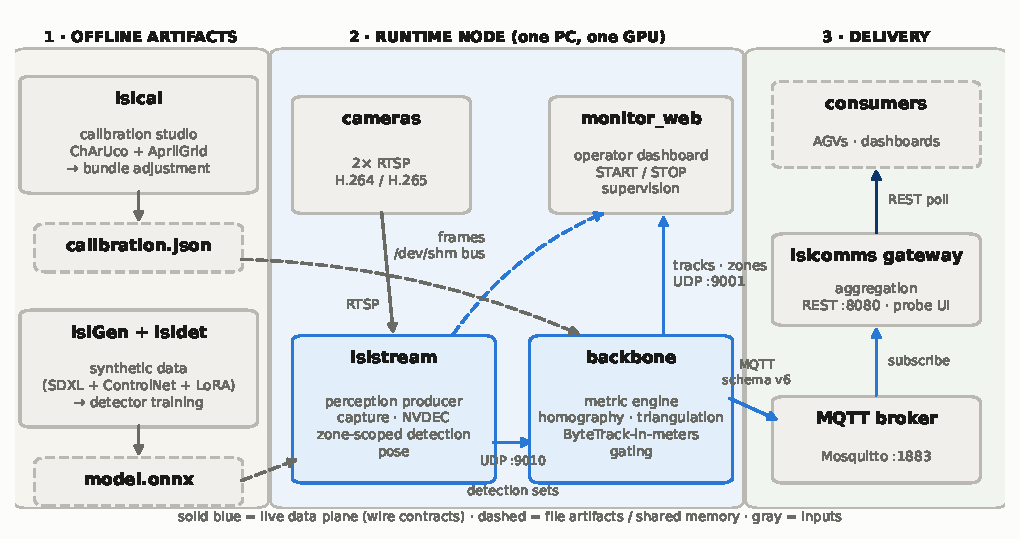
\includegraphics[width=0.92\textwidth]{figures/F1_architecture.pdf}
    \caption{Five-module architecture and the two frozen wire contracts: isistream $\to$ engine (per-camera detection sets, UDP loopback); engine $\to$ consumers (versioned UDP/JSON + MQTT); isicomms MQTT-in/REST-out for AGVs. isical and isiGen/isidet contribute only file artifacts (\texttt{calibration.json}, \texttt{.onnx}).}
    \label{fig:arch}
\end{figure*}

At runtime, the architecture is intentionally divided into two processes connected through a loopback interface (``Direction 1''). The separation reflects their contrasting computational characteristics: perception is GPU-intensive and throughput-oriented, whereas metric reasoning is CPU-light and latency-sensitive. Combining both within a single Python process introduced contention between the interpreter lock and inference thread pools, as quantified in Section 4.1. Accordingly, isistream performs frame capture, zone-aware detection, and pose estimation before transmitting a \texttt{DetectionSetMessage} for each camera to the backbone metric engine through a dedicated UDP loopback port (default 9010) --- the configuration referred to as \emph{points mode}. The engine therefore operates exclusively on detection metadata and imports neither CUDA runtimes nor inference libraries.

Each \texttt{DetectionSetMessage} carries four pieces of runtime information. First, it includes the frame \texttt{capture\_ts}, which serves as the single latency reference propagated through all downstream messages. When the motion gate (Section 2.4) suppresses inference, cached detections are re-emitted using the current frame's capture timestamp to preserve temporal continuity. Second, the producer transmits an explicit-empty heartbeat even when no objects are detected, allowing the engine to distinguish an empty scene from producer failure; message silence is therefore interpreted as a camera fault. Third, every message contains a per-camera monotonic sequence counter, enabling packet loss to be detected as measurable gaps despite UDP transport. Finally, a configuration fingerprint identifies inconsistencies in calibration, detection models, or monitoring zones between the producer and the metric engine.

To avoid redundant video decoding, decoded frames are distributed through a decode-once shared-memory frame bus. Frames from each camera are written into a dedicated shared-memory segment (\texttt{/dev/shm/isi3d\_frame\_<cam>}) implemented as a double-buffered seqlock with lock-free readers. This design eliminates duplicate RTSP sessions and decoding operations while ensuring that all consumers --- including the operator dashboard and future applications --- observe the exact same pixel data processed by the perception pipeline.

Inter-process communication relies on two stable interfaces: the backbone UDP/JSON schema (Section 2.7) and the isicomms MQTT-in/REST-out interface. Modules exchange information exclusively through these message contracts rather than shared code, allowing each component to evolve independently by extending the communication schema. Within the backbone itself, extensibility is restricted to five abstract plugin interfaces --- \texttt{FrameSource}, \texttt{Detector}, \texttt{Tracker}, \texttt{Triangulator}, and \texttt{MetadataSink} --- whose implementations self-register through a plugin registry. A dedicated unit test enforces the fixed set of extension points. All remaining components, including projection, fusion, gating, and stabilization, are implemented as concrete classes, limiting substitution to functionality where algorithmic or hardware diversity is genuinely required.

\subsection{Calibration --- isical}

Calibration transforms a newly installed camera system into a metrically accurate sensing rig and is designed to be performed by site operators using only printed planar calibration targets, without surveying equipment or computer vision expertise. The procedure is executed once per deployment and produces a single \texttt{calibration.json} file containing, for each camera, the intrinsic matrix $\mathbf{K}$, distortion coefficients $\mathbf{D}$ (OpenCV model), camera pose $(\mathbf{R}, \mathbf{t})$ in a common world coordinate system, and two runtime quantities derived from these parameters: the ground-plane homography $\mathbf{H}$ and the projection matrix $\mathbf{P}$. Both runtime geometric methods query this single calibration file, satisfying the ``one calibration, two queries'' invariant introduced in Section 2.5.

The stereo calibration workflow consists of two sequential stages, with each calibration target used where it provides the highest accuracy. Separating intrinsic and extrinsic estimation prevents errors in one stage from compensating for those in the other.

\textbf{Stage 1 --- Intrinsic calibration.} Each camera is calibrated independently using multiple handheld views of a ChArUco board ($5 \times 7$ squares, 120\,mm square length, 89.1\,mm marker length, \texttt{DICT\_5X5\_50}). The dense checkerboard corners provide well-conditioned intrinsic estimation. For the deployed system, 25 accepted images were captured per camera.

\textbf{Stage 2 --- Extrinsic calibration.} Relative camera poses are estimated through joint bundle adjustment using synchronized image pairs of a multi-board AprilGrid target (6 boards, each containing two tags arranged in a $1 \times 2$ grid, 180\,mm tag length, 0.30 tag-spacing ratio, family \texttt{t36h11}) distributed throughout the shared field of view. The intrinsic parameters obtained in Stage 1 remain fixed during optimization (\texttt{multical calibrate --fix\_intrinsic}), preventing bundle adjustment from absorbing intrinsic errors into the camera poses. The deployed installation required eight synchronized image pairs. Bundle adjustment is performed using the Multical toolbox in an isolated software environment to avoid dependency conflicts with OpenCV.

Image acquisition quality is enforced automatically by the isical Studio application rather than relying on operator judgment. Each captured frame is accepted only if it satisfies four criteria: detection of at least 12 ChArUco corners (or four AprilGrid tags), a Laplacian variance of at least 80 to reject blurred images, a maximum allowable inter-frame motion to ensure stability, and a novelty criterion that rejects near-duplicate board poses.

The generated calibration is validated before being written to disk. Two acceptance thresholds are enforced: a maximum per-camera reprojection RMS error of 0.5\,px for single-stage calibration and 2.0\,px for the two-stage joint extrinsic optimization, the latter matching the homography-error KPI defined in the customer specification. Any solution exceeding the applicable threshold is rejected, preventing an invalid calibration from entering production.

Although bundle adjustment estimates the relative poses of all cameras, it does not establish their position with respect to the warehouse floor. A separate floor-anchoring procedure therefore defines the global world coordinate system. The ChArUco board is placed flat on the floor at multiple locations (eight placements per camera in the deployed system). Each placement yields a board pose through PnP estimation (\texttt{cv2.solvePnP}), after which a RANSAC plane fit (inlier threshold 0.03\,m) is computed over all estimated planes. The resulting consensus plane defines the world plane ($Z = 0$), while the world origin and axes are taken from the first placement projected onto this plane. Using multiple placements prevents a single poorly positioned target from biasing the global reference frame.

For single-camera installations, where stereo bundle adjustment is unnecessary, the floor homography is estimated directly from operator-measured pixel-to-floor correspondences (Mode 1, Section 2.5). Although four non-collinear points are sufficient, five or more correspondences are recommended so that the estimation becomes overdetermined. Calibrations with a worst-case residual exceeding 0.10\,m are rejected, allowing incorrectly measured points to be detected automatically.

The stored camera pose $(\mathbf{R}, \mathbf{t})$ maps camera coordinates into the world coordinate system. Runtime projection instead uses its inverse, $\mathbf{R}' = \mathbf{R}^{\top}$, $\mathbf{t}' = -\mathbf{R}^{\top}\mathbf{t}$, so that a homogeneous world point $\mathbf{X} = (X, Y, Z, 1)^{\top}$ projects into image coordinates $\mathbf{p} = (u, v, 1)^{\top}$ as
\begin{equation}
s\,\mathbf{p} = \mathbf{P}\,\mathbf{X}, \qquad
\mathbf{P} = \mathbf{K}\,[\,\mathbf{R}' \mid \mathbf{t}'\,].
\end{equation}
Let $\mathbf{R}' = [\mathbf{r}_1\ \mathbf{r}_2\ \mathbf{r}_3]$. For points lying on the warehouse floor ($Z = 0$),
\begin{equation}
s\,\mathbf{p} = \mathbf{K}\,[\,\mathbf{r}_1\ \ \mathbf{r}_2\ \ \mathbf{t}'\,]
\begin{pmatrix} X \\ Y \\ 1 \end{pmatrix}
\;\triangleq\; \mathbf{H}_{w \to p} \begin{pmatrix} X \\ Y \\ 1 \end{pmatrix},
\qquad
\mathbf{H} = \mathbf{H}_{w \to p}^{-1},
\end{equation}
allowing undistorted image points to be mapped directly into metric floor coordinates. Lens distortion is handled separately: image points are first undistorted using $(\mathbf{K}, \mathbf{D})$ before the homography is applied (Section 2.5). Calibration quality is finally inspected in a 3D visualization tool that displays camera and calibration-target poses together with per-view reprojection errors (\figref{fig:calibration}).

\begin{figure*}[tbp]
    \centering
    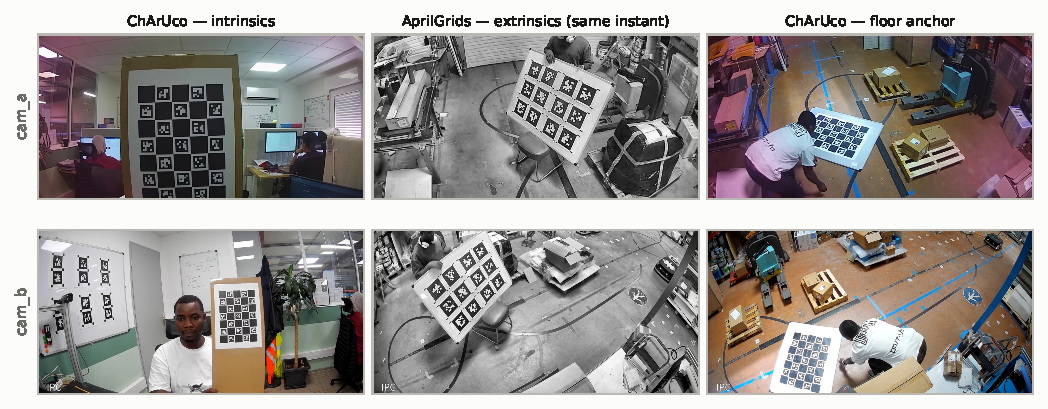
\includegraphics[width=0.9\textwidth]{figures/F3_calibration.pdf}
    \caption{Calibration materials and verification --- ChArUco and multi-AprilGrid boards as deployed, and the bundle-adjustment viewer showing camera/board poses with reprojection-error visualization.}
    \label{fig:calibration}
\end{figure*}

\subsection{Perception --- isistream and detection models}

isistream is the perception producer of isiMonitor3d. It owns the complete pixel-processing pipeline --- from RTSP video acquisition through object detection and pose estimation --- and converts each incoming frame into the compact detection sets consumed by the backbone metric engine (Section 2.2).

\textbf{Capture pipeline.} Each camera is ingested over RTSP (TCP transport) through a GStreamer pipeline constructed programmatically using PyGObject (Section 2.1). At startup, the stream codec is detected automatically and the pipeline instantiates the corresponding depayloader (H.264 or H.265/HEVC). Unlike automatic GStreamer plug-in selection, this explicit configuration supports mixed-codec camera installations while eliminating pad-linking race conditions.

Video decoding uses NVIDIA NVDEC hardware acceleration whenever available (\texttt{nvh264dec}/\texttt{nvh265dec}), including GPU-based color conversion and in-pipeline downscaling. When hardware acceleration is unavailable, decoding falls back automatically to software. The pipeline terminates in an appsink configured to retain only the newest decoded frame (\texttt{max-buffers=1, drop=true}). Since warehouse monitoring requires decisions based on the current scene rather than historical frames, discarding stale frames bounds end-to-end latency by design.

Each frame receives a \texttt{capture\_ts} timestamp immediately upon arrival at the appsink, representing the earliest instant at which the system observes the frame. This timestamp serves as the common temporal reference throughout the remainder of the processing pipeline. Relative to the physical scene, it includes the RTSP jitter-buffer delay (approximately 100\,ms) together with the video decoding latency, and therefore forms the basis of all latency measurements reported in Section 3.

\textbf{Runtime perception pipeline.} The perception pipeline executes as a paced processing loop. During each iteration, isistream:

\begin{enumerate}
    \item acquires the most recent frame and corresponding \texttt{capture\_ts} from every camera;
    \item performs zone-scoped object detection across all cameras using a single batched inference;
    \item executes person-pose estimation every $n$-th iteration, where $n$ is a configurable stride; and
    \item publishes one \texttt{DetectionSetMessage} per camera.
\end{enumerate}

Messages are transmitted even when no objects are detected, allowing downstream components to distinguish an empty scene from communication failure. Frames that become stale before processing are discarded, in which case no message is produced and the backbone treats the camera as unavailable.

\textbf{Motion gate.} Warehouse environments remain static for long periods, making repeated neural-network inference unnecessary. Since, for compact detection models, per-inference launch overhead is significant relative to arithmetic cost, reducing inference frequency provides a performance lever complementary to accelerating individual inferences.

Accordingly, each camera employs a motion gate (enabled in the deployed configuration). Motion is estimated using a lightweight grayscale signature computed from a $32 \times 32$ downsampled image. A frame is considered changed when more than 2\,\% of pixels differ by at least 15 grayscale levels.

Two independent motion gates operate for every camera. Object detection uses signatures computed separately for each monitoring zone so that movement outside operational areas does not trigger inference, whereas person-pose estimation evaluates motion over the full frame to preserve complete personnel monitoring. To prevent gradual drift, inference is forced periodically every two seconds (configurable).

Whenever inference is skipped --- or between pose-estimation stride intervals --- the previously inferred detections, including bounding boxes and segmentation polygons, are re-emitted using the current \texttt{capture\_ts}. Consequently, downstream consumers receive a continuous observation stream, while the backbone metric engine repeatedly updates its Kalman filters with the most recent valid measurements under the assumption that the scene remains unchanged. The motion-gate configuration and pose stride used during evaluation are reported in Section 3.

\textbf{Zone-scoped detection.} Zone scoping exploits the fixed-camera assumption introduced in Section 1. Because most of each warehouse image contains static floor or shelving, object detection is restricted to operator-defined floor regions, whereas the person-pose model continues to process the entire frame to ensure complete personnel coverage.

During system configuration, the operator declares each monitoring zone by clicking a small number of points (three or more; rectangular zones from two corners) either on the metric floor map or directly on either camera's live view; camera clicks are back-projected to the floor through the same undistortion and homography used by the runtime pipeline. Every zone is therefore stored once, as a floor polygon in metric coordinates --- the single source of truth from which all camera-specific geometry is derived. Using the calibration parameters, every polygon is projected into each camera view while accounting for lens distortion and extruded vertically between $z = 0$\,m and $z = 2$\,m, ensuring that the full height of loaded pallets remains inside the resulting crop; the projected outline is also displayed on every camera view, so the operator sees the same zone on both feeds regardless of where it was drawn. Zones outside a camera's field of view generate no crop.

At runtime, all visible zone crops from every camera are resized by letterboxing to a fixed detector input size (384\,px by default; 320\,px in the deployed system and throughout the experiments reported in Section 3) before being processed together in a single batched inference. The resulting detections are subsequently transformed back into full-frame image coordinates. This approach implicitly magnifies distant zones, allowing small objects to occupy a larger fraction of the detector input than they would in the original full-resolution image.

Because vertically extruded zones may overlap in image space, the same object can occasionally be detected in multiple crops. A per-camera, per-class cross-crop deduplication stage therefore retains only the highest-confidence detection. When no monitoring zones are configured, the object detector is omitted entirely and the system operates in pose-only mode.

\textbf{Cross-camera zone twins.} Because each zone is defined in metric floor coordinates, projecting it into the second camera materializes a \textit{twin}: the same physical floor region observed independently from both viewpoints, each with its own crop and its own detection inference. This redundancy is the zone mechanism's occlusion defense --- when a forklift or load blocks one camera's view of a zone, the other camera's twin continues to produce detections, so the zone's tracks and its retained occupancy state (\texttt{ZoneState}, Section 2.7) remain valid rather than lapsing; the two observation streams are reconciled downstream by the metric fusion stage (Section 2.5), which merges them when both cameras see an object and falls back to the surviving view when they do not. The operator dashboard derives each twin's outline automatically by round-tripping the drawn polygon through the floor plane --- sampling along its edges, since a straight image edge maps to a curve under lens distortion --- and regenerates all twins whenever the calibration changes. Segmentation masks are not transferred between cameras: each camera infers its own masks within its own crop, and only the zone geometry itself is projected across views.

\textbf{Detection models and inference runtime.} Object detection employs instance-segmentation networks from the two detector families introduced in Section 2.1: YOLO26-seg and RF-DETR-seg. All models are exported to ONNX and executed using ONNX Runtime. Using framework-independent ONNX models rather than vendor-specific engine formats allows identical model files to be deployed on both the development workstation and Jetson production hardware (Section 2.7), while hardware-specific acceleration is provided transparently through interchangeable execution providers.

On NVIDIA systems, in the configuration measured in this article (July 2026), inference used ONNX Runtime's TensorRT execution provider with compiled engines cached on disk. An optional slicing-assisted inference (SAHI) mode subdivides unusually large or elongated zone crops into overlapping square tiles before detection. Because TensorRT generates separate optimized engines for different input dimensions and SAHI introduces variable batch sizes, batches are padded into predefined buckets (1, 2, 4, 8, 16, and 32) to limit the total number of compiled engines.

The same detector interface also supports the CUDA execution provider as a fallback on NVIDIA GPUs, while an OpenVINO-based detector plugin behind the same interface enables deployment on Intel CPUs and integrated GPUs without modifying the remainder of the perception pipeline.

Person pose estimation is performed using a YOLO11-pose ONNX model. Each detected person includes 2D keypoints $(x, y, \text{confidence})$, from which the ankle midpoint is extracted as the representative foot point used by the geometric processing stage. Segmentation masks are polygonized and, together with bounding boxes, foot points, and keypoints, serialized into the per-camera \texttt{DetectionSetMessage}.

\subsection{Geometric core --- the backbone metric engine}

The backbone metric engine is where image measurements become metric object trajectories. It implements the two complementary geometric methods introduced in Section 2.1 behind a common calibration and a unified identity space (\figref{fig:pipeline}). Two architectural invariants govern its design. \textbf{One calibration, two queries:} both the homography-based and triangulation-based geometric pipelines read the same \texttt{calibration.json} file, ensuring that both methods operate from identical camera parameters. \textbf{One identity space:} track identities are created exclusively by the 2D tracker. The 3D pipeline never performs independent data association or re-identification; instead, it augments existing 2D tracks with three-dimensional coordinates.

\begin{figure*}[tbp]
    \centering
    
\includegraphics[width=0.92\textwidth]{figures/F2_pipeline.pdf}
    \caption{The geometric pipeline: always-on homography chain (foot point $\to$ undistortion $\to$ $\mathbf{H}$ $\to$ fusion $\to$ disagreement gate $\to$ ByteTrack-in-meters $\to$ stabilizer $\to$ \texttt{Track2D}) and subscription-driven triangulation branch (association $\to$ two-view DLT $\to$ reprojection gate $\to$ 3D Kalman $\to$ \texttt{Track3D}); shared calibration and identity space highlighted.}
    \label{fig:pipeline}
\end{figure*}

\textbf{Frame synchronization and operating modes.} Incoming per-camera \texttt{DetectionSetMessage}s (or decoded frames in the single-process fallback mode) are synchronized using an approximate-time policy based on \texttt{capture\_ts}. Whenever the oldest buffered frame from every camera falls within a configurable skew tolerance (33\,ms by default, corresponding to one frame at 30\,fps), the synchronizer emits a temporally aligned multi-camera observation.

The engine supports two operating modes determined by the configured number of cameras. \textbf{Mode 1 (single camera):} only the homography pipeline is instantiated, producing \texttt{Track2D}. \textbf{Mode 2 (stereo):} the homography pipeline continuously produces \texttt{Track2D}, while the triangulation pipeline generates \texttt{Track3D} whenever requested.

If one camera fails during stereo operation, the synchronizer waits for a 100\,ms grace period before switching automatically to single-camera processing. Buffered stale frames are discarded and only the latest frame from the surviving camera is processed thereafter. Consequently, \texttt{Track2D} continues uninterrupted, \texttt{Track3D} suspends automatically because its two-camera subscription condition is no longer satisfied, and object identities remain unchanged throughout degradation and recovery. The objective is graceful degradation rather than service interruption.

\textbf{Homography pipeline (always active).} The homography pipeline continuously estimates metric floor positions for every detected object. For each detection, only the foot point is projected onto the ground plane: the bottom-center of the bounding box for general objects and the ankle midpoint for persons. Since this point corresponds to the object's physical contact with the floor, it is the only image measurement geometrically consistent with planar projection.

The observed pixel $\mathbf{u}$ is first undistorted using the intrinsic calibration before being mapped into metric floor coordinates,
\begin{equation}
\begin{pmatrix} X \\ Y \\ 1 \end{pmatrix} \propto \mathbf{H}\,\tilde{\mathbf{p}},
\qquad \tilde{\mathbf{p}} = \Pi^{-1}(\mathbf{u};\, \mathbf{K}, \mathbf{D}),
\end{equation}
where $\Pi^{-1}$ denotes OpenCV undistortion.

When multiple cameras observe the same object --- including the two independent views of a twinned zone (Section 2.4) --- floor observations are fused before tracking. Candidate correspondences are obtained by solving a Euclidean-distance assignment problem in metric space using the Hungarian algorithm. Per-class matching thresholds (0.8\,m for persons and pallets, 1.6\,m for forklifts by default) determine whether observations represent the same physical object. Accepted pairs are merged by averaging their positions, whereas unmatched detections remain valid single-camera observations to accommodate partial occlusions.

A second, more conservative agreement gate verifies each merged observation. If the estimated positions disagree beyond tighter per-class thresholds (0.4\,m for persons and pallets, 0.8\,m for forklifts), fusion is rejected. The higher-confidence observation is retained while the conflicting measurement is discarded, implementing the system's ``fail honestly'' principle within the 2D pipeline.

\textbf{Metric-space tracking.} The fused observations are tracked using a modified ByteTrack implementation operating directly in metric coordinates. Unlike conventional image-space tracking, metric-space tracking makes association thresholds independent of camera geometry and enables all cameras to contribute to a single global tracker without requiring cross-camera identity reconciliation.

Each track maintains a constant-velocity Kalman filter with state $[X, Y, v_X, v_Y]$. Tracks are first predicted using the measured inter-frame interval before observations are divided into high- and low-confidence sets (default confidence thresholds: 0.5 and 0.1). Observations below the lower threshold are discarded.

Association proceeds through two Hungarian-assignment stages. Unlike the original ByteTrack formulation, the first stage matches all active tracks --- tracked, newly created, and previously lost --- to high-confidence detections. Remaining unmatched tracks are subsequently associated with low-confidence detections. Matching uses the Mahalanobis distance,
\begin{equation}
d^2(\mathbf{z}, \hat{\mathbf{z}}) = (\mathbf{z} - \hat{\mathbf{z}})^{\top} \mathbf{S}^{-1} (\mathbf{z} - \hat{\mathbf{z}}),
\end{equation}
where $\mathbf{S}$ is the innovation covariance of the Kalman filter. Unmatched high-confidence observations initialize new tracks. Track identifiers are assigned once and are never reused, preserving identity continuity even during temporary single-camera operation.

To suppress frame-level classification fluctuations, each track's semantic label is stabilized using majority voting over a sliding observation window. Tracks may additionally remain unpublished until they satisfy a configurable confirmation period. The resulting trajectories constitute the continuously published \texttt{Track2D} stream.

A parallel rule-based module estimates pallet occupancy by combining two complementary cues --- image overlap and metric floor margin --- which exhibit different failure modes. The resulting empty/full state is stabilized using the same temporal majority-voting mechanism.

\textbf{Triangulation pipeline (on demand).} Three-dimensional reconstruction is performed only for tracks satisfying declarative subscription rules, including object class, minimum number of observing cameras, zone membership, and optional per-track rate limits. This subscription-based design ensures that computational cost scales with consumer demand rather than scene complexity, since most industrial monitoring tasks require only floor-plane trajectories.

For every subscribed \texttt{Track2D}, the triangulation pipeline first resolves the corresponding image observations by matching floor projections back to the original per-camera detections from the same synchronized frame. Consequently, the triangulator performs only geometric reconstruction while inheriting object identities directly from the 2D tracker.

Stereo reconstruction uses the standard Direct Linear Transform (DLT) implementation (\texttt{cv2.triangulatePoints}). Each camera $i$, with projection matrix $\mathbf{P}_i$ and undistorted observation $\mathbf{p}_i$, contributes two linear equations,
\begin{equation}
[\mathbf{p}_i]_{\times}\, \mathbf{P}_i\, \mathbf{X} = \mathbf{0},
\end{equation}
which are solved jointly by singular value decomposition, with the reconstructed point corresponding to the singular vector associated with the smallest singular value.

Each reconstructed point is subsequently validated through reprojection. The estimated 3D point is projected back into every contributing camera, and reconstruction is rejected whenever the maximum reprojection error,
\begin{equation}
e_i = \left\lVert \pi(\mathbf{P}_i \hat{\mathbf{X}}) - \mathbf{p}_i \right\rVert_2,
\end{equation}
exceeds 5 pixels by default (the customer specification permits thresholds between 5 and 8 pixels).

Accepted observations update a second constant-velocity Kalman filter with state $[X, Y, Z, v_X, v_Y, v_Z]$, indexed by the corresponding \texttt{Track2D} identifier. Filters whose associated 2D tracks disappear are removed automatically during each update cycle. The resulting \texttt{Track3D} stream therefore carries exactly the same identities as \texttt{Track2D}, differing only in the addition of metric height information.

With only two cameras, the DLT system is exactly determined, limiting the types of geometric inconsistencies detectable through reprojection error alone. This limitation, together with the role of the upstream disagreement gate in mitigating it, is discussed in Section 4.

\subsection{Synthetic training data --- isiGen}

isiGen addresses the primary deployment bottleneck identified in Section 1: the collection and manual annotation of site-specific training data. Rather than relying solely on large annotated datasets, it expands a small collection of real photographs into a fully labeled synthetic dataset using the diffusion-based generation pipeline introduced in Section 2.1.

The pipeline consists of ten sequential stages implemented as independent plugins: curation, automatic detection, mask generation, control-map generation, captioning, LoRA training, scaffold synthesis, image generation, quality filtering, and dataset export.

The process begins by curating real images while preserving their original warehouse environments. Automatic object detection provides bounding-box prompts that seed mask generation, after which SAM2 produces color-coded segmentation masks. DepthAnythingV2 monocular depth estimation generates the depth control maps used to constrain image synthesis (a Canny edge extractor also runs at this stage, but its maps do not condition generation). Image captions are automatically constructed using a unique trigger token for each object class together with detailed background descriptions, reducing concept bleed during diffusion-based generation.

Class-specific LoRA adapters are then fine-tuned on Stable Diffusion XL, using an fp16 UNet with fp32 LoRA weights. For the black-polybag dataset, training used rank 16, a resolution of 768\,px, 2{,}000 optimization steps, a learning rate of $10^{-4}$, batch size 1 with four-step gradient accumulation, and 53 real training photographs.

Synthetic image generation combines Stable Diffusion XL, a depth-conditioned ControlNet, and the trained LoRA adapter. Generation is guided by procedurally synthesized scaffolds consisting of paired control maps and ground-truth segmentation masks, which may optionally be created by compositing real object instances onto empty warehouse backgrounds. The scaffold constrains scene geometry, while the text prompt randomizes object appearance and environmental variation, producing images whose annotations are known by construction. For the black-polybag dataset, 500 scaffolds and 553 captions produced 500 synthetic images, which were filtered using CLIP similarity scores before being exported in YOLO-seg format (\figref{fig:isigen}).

\begin{figure*}[tbp]
    \centering
    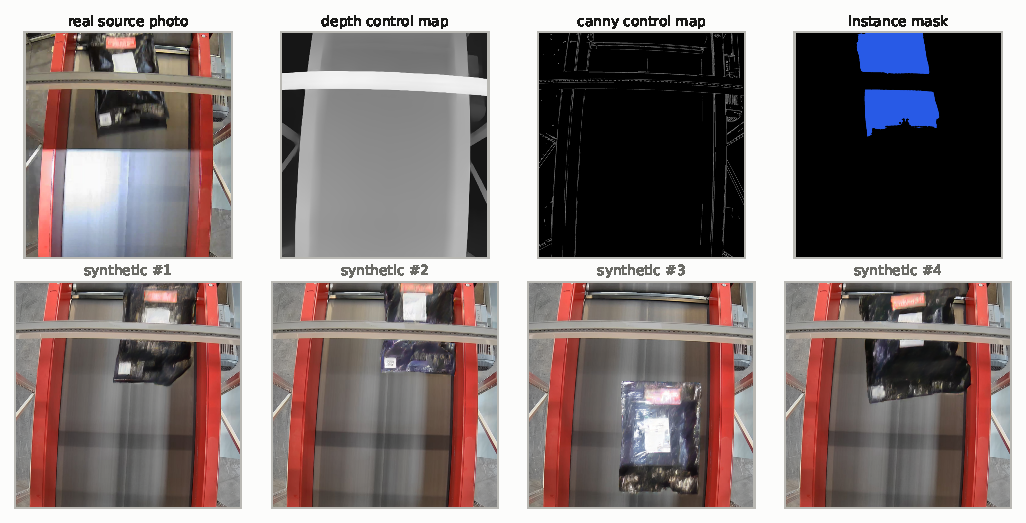
\includegraphics[width=0.9\textwidth]{figures/F4_isigen.pdf}
    \caption{isiGen samples --- real photograph, derived control map and ground-truth mask scaffold, and synthetic variants generated under geometric control with randomized appearance.}
    \label{fig:isigen}
\end{figure*}

The exported datasets are consumed by isidet, a dedicated training framework executed in a separate Conda environment. Isolating the training stack from the runtime environment ensures that training dependencies cannot affect the deployed perception system. isidet fine-tunes the YOLO26-seg and RF-DETR-seg models described in Section 2.4 and exports raw-head ONNX models for deployment.

The detector models evaluated in this work were trained exclusively on a real-image dataset comprising three object classes (\texttt{palette}, \texttt{carton}, \texttt{polybag}), containing 5{,}540 training images and 1{,}049 validation images. The synthetic images generated by isiGen were packaged into a separate merged dataset and were not used for the detector results reported in this paper. Instead, their contribution is evaluated independently through the training ablation study presented in Section 3.4.

\subsection{Communication and deployment}

The delivery layer converts the metric engine outputs into machine-readable interfaces for three categories of consumers: co-located software modules, remote or multi-node subscribers, and polling-based vehicle controllers. Each communication mechanism is selected according to the requirements of its target consumer.

All engine outputs crossing process boundaries are transmitted as Pydantic-validated JSON envelopes (schema version 6). Each message contains the schema version, message type, and originating \texttt{capture\_ts} timestamp, ensuring consistent temporal interpretation across all consumers. The message catalogue includes \texttt{Track2D}, \texttt{Track3D}, zone entry/exit events, image references, persistent zone states (\texttt{ZoneState}, used as the WMS/FMS integration signal), per-camera observations, incoming \texttt{DetectionSetMessage}s (Section 2.2), oversized-message fragmentation envelopes, proximity alerts, periodic diagnostic heartbeats, and retained configuration advertisements.

For low-latency communication between components deployed on the same site, the system uses UDP/JSON as the primary intra-site transport. Remote and multi-node consumers are served through MQTT, which provides broker-mediated distribution and retained message delivery. MQTT topics follow the hierarchy \texttt{<base>/<version>/<node\_id>/<suffix>}; the complete per-node topic tree is:

{\footnotesize
\begin{verbatim}
{prefix} = isiMonitor3D/v1/<node>
├─ track2d/{cls}          metric floor tracks
├─ track3d/{cls}          on-demand 3D tracks
├─ zone/{zone}            zone occupancy
│  │                        (retained, QoS 1)
│  ├─ passings            entry/exit events
│  └─ images/{track_id}   snapshot references
├─ proximity              person-object pairs
│                           (retained, QoS 1)
├─ diagnostics/heartbeat  node health heartbeat
└─ config                 config advertisement
                            (retained)
\end{verbatim}
}

\noindent This is the same hierarchy the isicomms probe interface renders live --- latest message per topic --- during commissioning. The MQTT topic version is intentionally independent from the payload schema version, allowing communication routing and message evolution to progress independently.

The isicomms module provides the interface between the internal messaging system and external industrial clients. It combines an MQTT broker (port 1883) with a REST gateway for polling-based consumers such as AGV fleet controllers. The gateway exposes an optionally token-authenticated HTTP API on port 8080 with endpoints for nodes (\texttt{/nodes}), zones (\texttt{/zones}), tracks (\texttt{/tracks}), and passing events (\texttt{/passings}). This abstraction avoids requiring vehicle controllers to implement MQTT clients, which is often incompatible with existing fleet-control software.

\textbf{Runtime environment and deployment.} Development and experimental evaluation are performed on a Linux/WSL2 workstation equipped with an NVIDIA RTX 5070 GPU (12\,GB, Blackwell architecture, sm\_120). The software stack consists of Python 3.10, OpenCV 4.13, GStreamer 1.28, and ONNX Runtime 1.23.2 with GPU acceleration through TensorRT 10.16 and CUDA 12.9.

The production deployment target is an NVIDIA Jetson Orin NX 16\,GB module (Seeed reComputer J4012). Python 3.10 is maintained to match the JetPack 6.x software environment. Since the runtime operates on framework-independent ONNX models through ONNX Runtime, which provides a Jetson-compatible backend, migration from development hardware to edge deployment requires only an environment change rather than modifications to application code.

In deployment, the perception producer and metric engine execute as two independent systemd-managed services sharing the same configuration file. This provides deterministic startup, automatic recovery after failure, and fully local operation without dependency on cloud infrastructure.

\section{Results}

All figures in this section trace to on-disk artifacts: the measurement-campaign records, training-run files, and the deployed calibration. Sample sizes and measurement conditions are stated with each table. This section reports observations only; interpretation follows in Section 4.

\subsection{Detector accuracy (validation split)}

\textbf{Data provenance.} A data-provenance audit of the training corpus, whose record is archived with the measurement artifacts, established two facts that frame every accuracy number below. First, the three-class corpus used for all reported detector training (\texttt{pallet3}: 5{,}540 training / 1{,}049 validation images; classes \texttt{palette}, \texttt{carton}, \texttt{polybag}) consists entirely of real photographs --- filename, byte-level hash, timeline, and visual checks found zero synthetic images in it. Second, the corpus has no independent held-out test split: the COCO-format \texttt{test} folder is a byte-identical duplicate of the validation folder, created only because the RF-DETR trainer requires the directory to exist. \textbf{All detector accuracy reported in this article is therefore validation-split accuracy}, and no test-split figures are given; the implications are discussed with the limitations in Section 4.

\textbf{Aggregate accuracy.} \tabref{tab:t1} reports the three detector configurations evaluated, all trained on \texttt{pallet3} under the isidet trainer (Section 2.6). For the RF-DETR run, which logs per-epoch metrics for both regular and exponential-moving-average (EMA) weights, we adopt the following checkpoint-selection rule, mirroring the YOLO trainer's own \texttt{best.pt} convention: \textbf{the EMA checkpoint of the epoch maximizing validation box mAP@0.5:0.95} (here epoch 23 of 41; the non-EMA metrics at the same epoch are 0.971 / 0.930).

\begin{table*}[tbp]
    \caption{Detector accuracy on the pallet3 validation split (1{,}049 real images, 1{,}436 instances; three classes).}
    \label{tab:t1}
    \centering
    \footnotesize
    \setlength{\tabcolsep}{3pt}
    \begin{tabular}{lccccccc}
    \toprule
    \textbf{Model (checkpoint)} & \textbf{Input} & \textbf{Box P} & \textbf{Box R} & \textbf{Box mAP@0.5} & \textbf{Box mAP@0.5:0.95} & \textbf{Mask mAP@0.5} & \textbf{Mask mAP@0.5:0.95} \\
    \midrule
    YOLO26l-seg (\texttt{best.pt}, epoch 154/172) & 640 & 0.950 & 0.951 & \textbf{0.977} & \textbf{0.948} & 0.972 & 0.921 \\
    YOLO26n-seg (\texttt{best.pt}, epoch 89/100) & 320 & 0.915 & 0.899 & 0.962 & 0.895 & 0.953 & 0.846 \\
    RF-DETR medium-seg (best-EMA, epoch 23/41) & 432 & 0.953 & 0.933 & 0.973 & 0.938 & 0.962 & 0.906 \\
    \bottomrule
    \end{tabular}
    \tabletext{Sources: YOLO26l row --- independent re-evaluation (command recorded in the measurement archive; \texttt{isi-train} env, ultralytics 8.4.22, torch 2.10.0+cu128, RTX 5070); YOLO26n row --- the run's \texttt{results.csv} at its best epoch; RF-DETR row --- the run's \texttt{metrics.csv} at the selected checkpoint.}
\end{table*}

\textbf{Reproduction.} The headline YOLO26l-seg numbers were regenerated from the stored \texttt{best.pt} by an independent validation pass on the same 1{,}049 images: box mAP@0.5 reproduced exactly (0.977) and box mAP@0.5:0.95 within 0.001 of the training-time report (0.948 vs 0.947); precision/recall differ slightly (0.950/0.951 vs 0.960/0.939) because the evaluator selects a different F1-optimal confidence point per run. The re-evaluation also recorded the mask mAPs (0.972 / 0.921), which the original training report did not headline. Evaluation speed in that pass was 1.2\,ms preprocess / 10.3\,ms inference / 1.2\,ms postprocess per image at batch 8. Raw outputs (PR curves, confusion matrices) are archived with the measurement artifacts.

\textbf{Per-class accuracy.} \tabref{tab:t2} gives the per-class breakdown of the independently re-evaluated YOLO26l-seg model; class--label mapping is taken directly from the dataset's \texttt{data.yaml} and is authoritative by construction.

\begin{table*}[tbp]
    \caption{YOLO26l-seg per-class validation accuracy (independent re-evaluation).}
    \label{tab:t2}
    \centering
    \small
    \setlength{\tabcolsep}{4pt}
    \begin{tabular}{lcccccccc}
    \toprule
    \textbf{Class} & \textbf{Images} & \textbf{Instances} & \textbf{Box P} & \textbf{Box R} & \textbf{Box mAP@0.5} & \textbf{Box mAP@0.5:0.95} & \textbf{Mask mAP@0.5} & \textbf{Mask mAP@0.5:0.95} \\
    \midrule
    palette & 808 & 1{,}047 & 0.973 & 0.945 & 0.989 & 0.933 & 0.974 & 0.895 \\
    carton & 74 & 174 & 0.909 & 0.948 & 0.960 & 0.943 & 0.960 & 0.900 \\
    polybag & 186 & 215 & 0.967 & 0.958 & 0.983 & 0.969 & 0.980 & 0.967 \\
    \bottomrule
    \end{tabular}
\end{table*}

For RF-DETR medium-seg, the trainer's COCO evaluator reports per-class box AP at the selected checkpoint of 0.916 (palette), 0.905 (carton), and 0.971 (polybag).

\textbf{KPI observation.} All three configurations exceed the mAP@0.5 $\geq 0.90$ acceptance target on the validation split (0.962--0.977); the smallest model does so at a 320\,px input.

\textbf{KPI coverage note.} The pallet empty/full classification target (precision/recall $\geq 0.95/0.93$) is \textbf{not validated in this work}: the two-estimator occupancy mechanism is implemented and deployed (Section 2.5), but no labeled empty/full evaluation was performed. This gap is recorded with the limitations in Section 4.

\subsection{Calibration accuracy}

The deployed two-camera rig (project \texttt{c1}) was calibrated with the two-stage workflow of Section 2.3: 25 accepted ChArUco shots per camera (intrinsics), 8 synchronized pairs of the 6-board AprilGrid target (extrinsics, intrinsics fixed), and 8 flat ChArUco floor placements per camera (world anchor, RANSAC consensus plane).

\begin{table}[tbp]
    \caption{Deployed-rig calibration reprojection RMS.}
    \label{tab:t3}
    \centering
    \footnotesize
    \begin{tabular}{>{\raggedright\arraybackslash}p{0.36\columnwidth}ccp{0.2\columnwidth}}
    \toprule
    \textbf{Quantity} & \textbf{cam\_a} & \textbf{cam\_b} & \textbf{Applicable gate} \\
    \midrule
    Intrinsic-stage reprojection RMS (25 shots/cam) & 0.603\,px & 0.451\,px & --- (feeds the fixed-K extrinsic solve) \\
    Joint extrinsic consensus reprojection RMS & 1.621\,px & 1.621\,px & $\leq 2.0$\,px (assembly gate) \\
    \bottomrule
    \end{tabular}
\end{table}

The written calibration passed the 2.0\,px assembly gate with a joint consensus RMS of 1.621\,px on both cameras (\tabref{tab:t3}). This bundle-adjustment residual is the quantity checked against the $\leq 2$\,px homography-error acceptance target at calibration time; its relation to runtime floor-projection error is discussed in Section 4. The intrinsic-stage values are the per-camera ChArUco solve residuals consumed, with intrinsics frozen, by the joint solve.

\subsection{End-to-end runtime}

\textbf{Live latency measurement.} End-to-end capture$\to$publish latency was measured on the live production system by passively recording its MQTT diagnostics heartbeat for 310\,s --- 61 heartbeats, each carrying the \texttt{LatencyMeter} percentiles over a rolling window of $n = 2{,}048$ published messages; no probe process touched the pipeline. System state at capture: the deployed default configuration (points mode with the isistream producer and metric engine as separate processes, motion gate enabled, pose stride 1 --- the pose model runs on every non-gated tick, \texttt{pose\_every\_n: 1} --- TensorRT execution provider, zone-scoped detection, both cameras alive, 25.8\,fps aggregate, frame count $> 18{,}000$), with the dashboard (\figref{fig:dashboard}, shown in a representative live session), MQTT broker, and gateway all running --- i.e., full production load. Whole-GPU memory under this load was 7.6 of 12.2\,GiB (a machine total across all processes, including the desktop and dashboard; WSL2 exposes no per-process VRAM attribution). Because the motion gate was active, its cached re-emissions (Section 2.4) are included in the measured distribution. Latency is defined against \texttt{capture\_ts}, whose clock definition and $\sim$100\,ms pre-appsink lag are stated in Section 2.4; the KPI is defined against this clock.

\begin{table}[tbp]
    \caption{Capture$\to$publish latency, live production system (median across 61 heartbeats; min--max over the 310\,s window).}
    \label{tab:t4}
    \centering
    \small
    \begin{tabular}{lcc}
    \toprule
    \textbf{Percentile} & \textbf{Latency} & \textbf{Range} \\
    \midrule
    p50 & \textbf{40.3\,ms} & 39.5 -- 42.1\,ms \\
    p95 & \textbf{78.1\,ms} & 76.2 -- 79.9\,ms \\
    p99 & \textbf{94.0\,ms} & 90.4 -- 102.4\,ms \\
    \bottomrule
    \end{tabular}
\end{table}

The p95 of 78.1\,ms (\tabref{tab:t4}) meets the $< 200$\,ms acceptance target with a $\times 2.6$ margin. Throughout the 310\,s window every heartbeat reported the dual-camera mode with both sources alive and balanced per-camera rates ($\approx$13.4--13.8\,fps per camera, $\approx$26\,fps aggregate; \figref{fig:latency}). An earlier configuration of the same system --- before the ingest downscale to 720p, the pose input-size reduction, and the motion gate were introduced --- had been measured at p50 77 / p95 126\,ms; that prior figure is retained here only to date the configuration change, and the live measurement above is the reported result.

\begin{figure}[tbp]
    \centering
    
\includegraphics[width=\columnwidth]{figures/F5_latency.pdf}
    \caption{Capture$\to$publish latency of the live production system over the 310\,s measurement window --- per-heartbeat p50/p95/p99 traces from the 61 diagnostics heartbeats, with the 200\,ms KPI line.}
    \label{fig:latency}
\end{figure}

\begin{figure*}[tbp]
    \centering
    
\includegraphics[width=0.85\textwidth]{figures/F6_dashboard.png}
    \caption{The operator dashboard of the deployed system in live operation (representative session) --- CAM 2 live view with two configured zone polygons (\texttt{Sortie\_1}, red dashed, holding a loaded pallet with a carton; \texttt{Sortie\_2}, yellow dashed, holding an empty pallet); a tracked person with pose skeleton and on-frame metric proximity distances (2.0\,m and 3.5\,m); per-zone occupancy cards driven by the MQTT zone-state stream, reporting live pallet empty/full state (``Palette pr\'esente avec carton'' / ``Palette pr\'esente mais vide''); per-zone detection panels with the zone crops and an instance-segmented carton (confidence 0.83); and start/stop controls with status and log panels.}
    \label{fig:dashboard}
\end{figure*}

\textbf{Execution-provider benchmark.} The production detector (\texttt{yolo26n-seg}, fp16 ONNX, three classes, mask decoding enabled as deployed) was benchmarked under the TensorRT and CUDA execution providers of ONNX Runtime 1.23.2 (TensorRT 10.16, CUDA 12.9, RTX 5070, WSL2), at the production input size (320) and at 640. Each (EP $\times$ size) configuration ran in its own process, strictly sequentially: $N = 50$ timed calls after 5 warm-ups, for both the isolated \texttt{session.run} (pure inference) and the full \texttt{detect()} call (preprocess + inference + detection decoding + mask assembly; the end-to-end head requires no NMS). The TensorRT engine cache was warm (detector build 1.0--1.9\,s; no engine compilation occurred), so the figures reflect steady-state production behavior. The operator dashboard held $\approx$5\,GB VRAM and was streaming throughout; medians are therefore the robust statistic, and occasional p95 spikes (e.g., CUDA-640 inference p95 62.6\,ms vs median 16.4\,ms) coincide with this background load.

\begin{table}[tbp]
    \caption{TensorRT vs CUDA execution provider ($N = 50$ per cell; medians).}
    \label{tab:t5}
    \centering
    \footnotesize
    \begin{tabular}{llcc}
    \toprule
    \textbf{Measurement} & \textbf{EP} & \textbf{320\,px} & \textbf{640\,px} \\
    \midrule
    Isolated inference (median ms) & CUDA & 13.85 & 16.39 \\
     & TensorRT & 4.55 & 5.83 \\
     & \textit{TRT speedup} & \textit{3.0$\times$} & \textit{2.8$\times$} \\
    \midrule
    Full \texttt{detect()} (median ms) & CUDA & 22.35 & 64.35 \\
     & TensorRT & 8.74 & 46.68 \\
     & \textit{TRT speedup} & \textit{2.6$\times$} & \textit{1.4$\times$} \\
    \midrule
    Bench VRAM footprint ($\Delta$ MB) & CUDA & 207 & 432 \\
     & TensorRT & 309 & 321 \\
    \bottomrule
    \end{tabular}
\end{table}

At 640\,px, the full-\texttt{detect()} gain collapses to 1.4$\times$ although the isolated-inference gain remains 2.8$\times$ (\tabref{tab:t5}): of the 46.7\,ms TensorRT median, $\approx$41\,ms is CPU-side work (letterboxing, fp16 conversion, detection decoding, and full-frame mask assembly with \texttt{decode\_masks=True}). VRAM deltas are the benchmark's own footprint over a $\approx$5\,GB baseline held by the concurrently running dashboard.

\subsection{Synthetic-data training ablation (polybag)}

The contribution of the isiGen synthetic data is measured by a single-class (polybag) instance-segmentation training ablation: three training arms with identical model and hyperparameters (\texttt{yolo26n-seg.pt}, 640\,px, 80 epochs, batch 8, fixed seeds), each evaluated on one common \textbf{real} test set never seen by any arm --- the 186 polybag-containing images of the pallet3 validation split (215 instances). Arm S (synthetic-only) trains on the 238 training images among the 267 CLIP-filtered SDXL+ControlNet+LoRA generations of the isiGen export (the remaining 29 form its validation split), with the 53 real LoRA-source photos explicitly excluded; Arm R (real-only) trains on a count-matched random subsample (seed 42) of the 737 polybag-containing pallet3 \textit{training} images; Arm R+S trains on their union. Each arm's checkpoint is its own \texttt{best.pt}, selected on that arm's validation split --- Arm S therefore selects on synthetic validation images, Arms R and R+S on their own splits. Leakage checks: the test set draws only from pallet3 \textit{val}, Arm R only from pallet3 \textit{train} (split preserved from the source dataset), the synthetic images share zero bytes with pallet3 (the provenance audit's hash/size intersection: 0 collisions), and an md5 intersection of the 53 real LoRA-source photos against the 186 test images found 0 overlaps (recorded in the ablation record) --- the generator never saw any test image.

\begin{table*}[tbp]
    \caption{Ablation on the common real test set (186 images, 215 polybag instances).}
    \label{tab:t6}
    \centering
    \small
    \setlength{\tabcolsep}{3pt}
    \begin{tabular}{lccccccc}
    \toprule
    \textbf{Arm} & \textbf{Train images (real/syn)} & \textbf{Box P} & \textbf{Box R} & \textbf{Box mAP@0.5} & \textbf{Box mAP@0.5:0.95} & \textbf{Mask mAP@0.5} & \textbf{Mask mAP@0.5:0.95} \\
    \midrule
    S (synthetic-only) & 0 / 238 & 0.319 & 0.391 & 0.223 & 0.185 & 0.219 & 0.179 \\
    R (real-only) & 238 / 0 & 0.922 & 0.885 & 0.941 & 0.927 & 0.946 & 0.930 \\
    R+S (merged) & 238 / 238 & 0.906 & 0.935 & \textbf{0.962} & \textbf{0.950} & 0.965 & 0.950 \\
    \bottomrule
    \end{tabular}
\end{table*}

All three trainings completed normally (exit code 0; 80 epochs each; 0.26\,h for Arm R and 0.50\,h for Arm R+S on the RTX 5070); raw per-run outputs and logs are archived with the measurement artifacts (\tabref{tab:t6}).

Three observations follow from the table. First, the synthetic-only model is a functioning detector on synthetic imagery --- on its own synthetic validation split it reaches box mAP@0.5 $\approx 0.936$ --- but transfers to real frames at 0.223 box mAP@0.5: a real-transfer drop of $\sim$0.71 mAP@0.5 for this class and pipeline configuration. Second, adding the 238 synthetic images to the 238 real ones raises every mAP metric on the real test set: box mAP@0.5 $+0.021$ (0.941 $\to$ 0.962), box mAP@0.5:0.95 $+0.023$ (0.927 $\to$ 0.950), mask mAP@0.5:0.95 $+0.020$ (0.930 $\to$ 0.950), and recall $+0.050$ (0.885 $\to$ 0.935), while precision moves from 0.922 to 0.906. Third, as a measurement condition, each arm ran with a single seed; differences of $\sim$0.02 mAP are within single-seed training noise for datasets of this size. The test set contains only polybag-positive real images from one site's camera family, so false positives on object-free frames are not measured here. Interpretation of these observations --- including how the R+S margins relate to the noise floor --- is deferred to Section 4.

\subsection{Geometric verification bounds (synthetic ground truth)}

The geometric core's accuracy is continuously verified against synthetic ground truth by the repository's hermetic end-to-end tests (721 tests collected on 2026-07-20); these are \textbf{software verification bounds under a synthetic camera model, not field accuracy measurements} --- no tape-measured ground-truth campaign has yet been run on the deployed rig (Section 4).

\begin{table}[tbp]
    \caption{Synthetic end-to-end accuracy bounds enforced by the test suite.}
    \label{tab:t7}
    \centering
    \footnotesize
    \begin{tabular}{>{\raggedright\arraybackslash}p{0.34\columnwidth}>{\raggedright\arraybackslash}p{0.25\columnwidth}>{\raggedright\arraybackslash}p{0.28\columnwidth}}
    \toprule
    \textbf{Path} & \textbf{Condition} & \textbf{Enforced bound} \\
    \midrule
    Homography chain (foot $\to$ \texttt{Track2D}) & zero pixel noise & $\leq 1$\,mm vs ground truth (asserted at $10^{-3}$\,m) \\
    Homography chain & 2\,px Gaussian noise on every detection & $< 10$\,cm vs ground truth \\
    Triangulation (foot centroid $\to$ \texttt{Track3D}) & zero pixel noise, 2 cameras & $\leq 1$\,mm in $X, Y, Z$ \\
    Reprojection gate & all triangulations & max per-view error $\leq 5$\,px (deployed default; 5--8\,px allowed) \\
    \bottomrule
    \end{tabular}
\end{table}

The bounds (\tabref{tab:t7}) are assertions in the repository's synthetic end-to-end homography and triangulation tests, exercised on every suite run; the pipeline under test is composed from the production classes (projector, fusion, gates, trackers, triangulator), not mocks.

\section{Discussion}

\subsection{Interpretation}

\textbf{Why the architecture meets the latency KPI.} The live latency result (p95 78.1\,ms under full production load, \tabref{tab:t4}) is attributable to the accumulated design choices of Section 2 rather than to any single optimization. The split-process design was motivated by development-log measurements made during the July 2026 migration, under a pre-campaign configuration: running perception in-process with the dashboard cost $\sim$2{,}200\,ms per perception tick versus $\sim$55\,ms standalone (interpreter-lock and ONNX Runtime thread-pool contention), and the points-mode engine reduced total VRAM from $\sim$5.2\,GB to $\sim$2.5\,GB. We report these figures as design rationale with their provenance stated: they are development measurements, not campaign artifacts, and the per-process VRAM split cannot be re-measured today because WSL2 exposes no per-process attribution --- the current whole-GPU figure under production load is 7.6 of 12.2\,GiB (Section 3.3). The improvement from the earlier configuration's p50 77 / p95 126\,ms to the measured 40.3 / 78.1\,ms reflects the combined introduction of the in-pipeline 720p downscale, the reduced pose input size, the motion gate, and the TensorRT provider; the per-lever decomposition was not isolated and we do not apportion it.

The $\times 2.6$ margin against the 200\,ms target must be read with the clock definition of Section 2.4: \texttt{capture\_ts} starts $\sim$100\,ms (jitter buffer plus decode) after the optical event. Optical-event-to-publish is therefore roughly 100\,ms larger than the reported figures; the KPI is met as defined against the specification's capture clock, and the remaining headroom is what the Jetson port will consume.

\textbf{Why 320\,px zone crops are the enabling choice.} The execution-provider benchmark shows TensorRT's isolated inference gain (2.8--3.0$\times$) collapsing to 1.4$\times$ end-to-end at 640\,px, because $\approx$41\,ms of the 46.7\,ms median is CPU-side letterboxing, decoding, and mask assembly (\tabref{tab:t5}); medians are used throughout this comparison because the benchmark ran beside the $\approx$5\,GB dashboard load (Section 3.3). At the deployed 320\,px the end-to-end gain remains 2.6$\times$. Zone scoping is what makes the small input viable: each zone crop receives more model pixels than it would occupy in a full frame (Section 2.4), so accuracy-relevant resolution is preserved while the postprocessing volume that throttles the GPU gain stays small. Conversely, further model acceleration at 640\,px would be unproductive without moving postprocessing off the CPU.

\textbf{What the ablation shows about synthetic data.} The training ablation supports reading the isiGen pipeline as an \textit{augmenter}, not a replacement for real data: the synthetic-only arm transfers to real frames at 0.223 box mAP@0.5 against 0.941 for the count-matched real arm --- a real-transfer drop consistent with an appearance domain gap (single site and camera family, CLIP filtering notwithstanding). The merged arm's mAP margins over real-only ($+0.021$/$+0.023$) lie within the stated $\sim$0.02 single-seed noise floor and are therefore consistent with a small benefit rather than established; the recall gain ($+0.050$) is the only movement plausibly outside the floor and is the effect we consider robust. Two design facts bound this reading: the merged arm trains on twice the images of the real arm, confounding ``synthetic data'' with ``more data'' (737 real images existed; an R-full arm would separate the confound), and the count-matched design represents the scarce-real-data scenario rather than this site's actual data budget. The decision-relevant experiment remains unrun: an arm of $\sim$53 real images with and without synthetic augmentation --- the actual fifty-photo deployment scenario claimed in Section 1.

\textbf{Calibration residual versus the homography KPI.} The 1.621\,px consensus figure (\tabref{tab:t3}) is a bundle-adjustment residual over board corners, not a direct measurement of runtime floor-projection error. It is a meaningful proxy --- the same $\mathbf{K}, \mathbf{R}, \mathbf{t}$ that generate the residual compose the runtime $\mathbf{H}$, so systematic calibration error would surface in both --- but it does not bound projection error on floor regions the boards never covered. A field check against surveyed floor points is required before the $\leq 2$\,px KPI can be considered verified in the runtime sense.

\subsection{Limitations}

\begin{enumerate}
    \item \textbf{Validation-split accuracy with validation-selected checkpoints.} No held-out test split exists (Section 3.1); \texttt{best.pt}/best-EMA checkpoints are selected on the same split that is reported, adding optimistic selection bias. Deployment-frame accuracy is unmeasured, and per-class support is imbalanced (carton: 74 images), widening per-class uncertainty.
    \item \textbf{Ablation scope.} The training ablation uses one seed per arm with margins at its $\sim$0.02 noise floor, one class, 238-image arms, a 186-image single-site positives-only test set (no false-positive measurement on object-free frames), a data-budget confound (476 vs 238 training images), and arm-local checkpoint selection.
    \item \textbf{No field geometric ground truth.} The planned live triangulation-error logging and tape-measure campaign were not run; geometric accuracy rests on synthetic verification bounds (\tabref{tab:t7}), and the 5\,px reprojection gate is a configured threshold, not a measured error distribution.
    \item \textbf{Two-camera gate blindness.} With exactly two cameras the DLT is exactly determined, so the reprojection gate cannot detect cross-camera disagreement at the 3D stage; mitigation is the upstream 2D disagreement gate, and the 3D gate becomes informative only with $\geq 3$ cameras.
    \item \textbf{Clock definition.} Reported latency excludes $\sim$100\,ms of pre-appsink pipeline (jitter buffer + decode); see Section 4.1.
    \item \textbf{Pallet empty/full KPI unvalidated.} The occupancy mechanism is deployed but no labeled precision/recall measurement exists (Section 3.1).
    \item \textbf{Platform.} All measurements were made on the development workstation (RTX 5070, WSL2); the Jetson Orin NX port is argued portable via the ONNX artifact, not demonstrated.
    \item \textbf{Single deployment.} One site, one rig, one camera family underlie every finding, including the calibration and ablation test data.
    \item \textbf{Motion-gate re-emissions in the latency distribution.} Gated (cached) ticks share the measured latency distribution with inferred ticks; worst-case always-inferring latency was not isolated.
\end{enumerate}

\section{Conclusions}

This article presented isiMonitor3d, an integrated industrial vision pipeline that turns one or two fixed cameras into metric, identity-stable warehouse monitoring, from operator-guided calibration to machine-consumable delivery. Against the customer acceptance targets, the measured outcomes are: end-to-end capture-to-publish latency of p95 78.1\,ms under full production load, within the $< 200$\,ms target as defined by the specification's capture clock; a calibration bundle-adjustment residual of 1.621\,px against the $\leq 2$\,px homography-error target, noting that this residual is a calibration-time proxy for the runtime projection error (Section 4.1); and detection mAP@0.5 of 0.962--0.977, above the $\geq 0.90$ target, on the validation split. Two targets remain unverified: the pallet empty/full precision/recall KPI (mechanism deployed, no labeled measurement) and field geometric accuracy (the triangulation gate is a configured threshold, not a measured error).

The contributions stand as follows. A modular five-module architecture with frozen communication contracts delivers single-decode, multi-consumer processing with the measured real-time performance above. A dual-method localization framework serves always-on ground-plane homography and on-demand stereo triangulation from a shared calibration and identity space. An operator-guided calibration workflow reaches the 1.62\,px reprojection consensus on the deployed rig using printed calibration boards only. A synthetic-data generation pipeline based on SDXL, ControlNet, and LoRA is evaluated quantitatively against real training data, its measured role being to augment, not replace, it.

Future work follows directly from the limitations. First, the field measurements not yet run: live triangulation reprojection-error logging and a tape-measured ground-truth campaign on the deployed rig. Second, the decision-relevant training experiments: the $\sim$53-real $\pm$ synthetic arm that tests the actual fifty-photo scenario, together with seed replication of the ablation. Third, the Jetson Orin NX port, argued portable through the shared ONNX artifact but not yet demonstrated. Fourth, extension to $\geq 3$ cameras via aniposelib triangulation, which makes the reprojection gate informative. Fifth, the deferred pose-mode extension, lifting per-keypoint 3D rather than the foot centroid alone.

%----------------------------------------------------------

\printbibliography

%----------------------------------------------------------

\end{document}
